\chapter{APMアルゴリズムの導出}
\label{sec:AMP}
\section{近似的確率伝播法 (Approximate Belief Propagetion BP)}
通信路推定とデータ推定のための確率伝播法(Belief Propagetion BP)から説明を開始する.因子ノード$y_{nt}$から変数ノード$x_{kt}$および,$h_{nk}$に渡されるメッセージをそれぞれ$m_{nt\to kt}(x_{kt})$と$m_{nt\to nk}(h_{nk})$とする.また,反対方向に渡されるメッセージをそれぞれ$q_{kt\to nt}(x_{kt})$,$q_{nk\to nt}(h_{nk})$とする(図\ref{fig:message}参照).
\begin{figure}[htbp]
  \begin{center}
    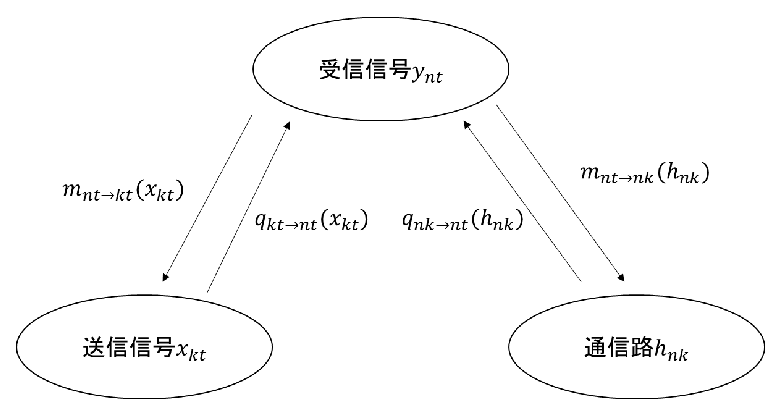
\includegraphics[clip,width=10.0cm]{./message.eps}
    \caption{メッセージの交換}
    \label{fig:message}
  \end{center}
\end{figure}

それぞれのメッセージは次のように更新される.
\begin{equation}
	\label{eq:message_x}
	m_{nt\to kt}(x_{kt}) = 
		\int 
			\frac{1}{\pi N_0}
			e^
			{
				-\frac
					{|y_{nt}-h_{nk'}x_{k't}-I_{n,k,u}|^2}
					{N_0}
			}
			\prod_{k'\neq k}
				q_{k't\to nt}(x_{k't})dx_{k't}
			\prod_{k'=1}^{K}
				q_{nk'\to nt}(h_{nk'})dh_{nk'} ,
\end{equation}
\begin{equation} 
	\label{eq:message_inv_x}
	q_{kt\to nt}(x_{kt}) \propto
		p(x_{kt})
		\prod_{n'\neq n}
		m_{n't\to kt}(x_{kt}) ,
\end{equation}
\begin{equation} 
	\label{eq:message_h}
	m_{nt\to nk}(h_{nk}) = 
		\int 
			\frac{1}{\pi N_0}
			e^
			{
				-\frac
					{|y_{nt}-h_{nk'}x_{k't}-I_{n,k,u}|^2}
					{N_0}
			}
			\prod_{k'\neq k}
				q_{nk'\to nt}(h_{nk'})dh_{nk'}
			\prod_{k'=1}^{K}
				q_{k't\to nt}(x_{k't})dx_{k't} ,
\end{equation}
\begin{equation} 
	\label{eq:message_h_inv}
	q_{nk\to nt}(h_{nk}) \propto
		p(h_{nk})
		\prod_{t'\neq t}
		m_{nt'\to nk}(h_{nk}) ,
\end{equation}
ここで,$I_{n,k,t}$は他のユーザからの干渉であり,次のように定義される.
\begin{equation}
	\label{eq:I}
	I_{n,k,t}=
		\frac{1}{\sqrt{N}}
		\sum_{k'\neq k}
			h_{nk'}x_{k't}	
		.
\end{equation}
なお,ここでは反復のスケジューリングについては指定していないことを明記しておく.

複雑さを軽減するため,大きなシステムを考え中心極限定理に従い,干渉のガウス近似を行うと,以下のような式が導出できる.
\begin{equation} 
	\label{eq:paramerter_start}
	\hat{x}_{kt\to nt} = 
		\int
			xq_{kt\to nt}(x)dx, \\
\end{equation}
\begin{equation} 
	\label{eq:paramerter_second}
	\xi_{kt\to nt} =
		\int
			|x-\hat{x}_{kt\to nt}|^2q_{kt\to nt}(x)dx,\\
\end{equation}
\begin{equation} 
	\hat{h}_{nk\to nt} =
		\int
			hq_{nk\to nt}(h)dh,\\
\end{equation}
\begin{equation} 
	\label{eq:paramerter_end}
	\eta_{nk\to nt} =
		\int
			|h-\hat{h}_{nk\to nt}|^2q_{nk\to nt}(h)dh.
\end{equation}
目標は,(\ref{eq:paramerter_start})~(\ref{eq:paramerter_end})の閉形式を導出することである.データ推定に関連するメッセージは以下のように示される.
\begin{equation}
	\label{eq:x_h_bp}
	\hat{x}_{kt\to nt} = 
		f_{k}(\Re[\overline{x}_{kt\to nt}];\overline{\xi}_{kt\to nt})
		+jf_{k}(\Im[\overline{x}_{kt\to nt}];\overline{\xi}_{kt\to nt}), 
\end{equation}
\begin{equation}
	\label{eq:xi_bp}
	\xi_{kt\to nt} = 1 - |\hat{x}_{kt\to nt}|^2, \\
\end{equation}
\begin{equation}
	\label{eq:x_mean}
	\overline{x}_{kt\to nt}= 
		\frac{\overline{\xi}_{kt\to nt}}{\sqrt{N}}
		\sum_{n'\neq n}
			\frac
				{\hat{h}^{*}_{n'k\to n't}(y_{n't}-\overline{I}_{n',k,t})}
				{N_0+\zeta_{n',k,t}}, \\
\end{equation}
\begin{equation}
	\label{eq:x_var}
	\overline{\xi}_{kt\to nt}=
		\left(
			\frac{1}{N}
			\sum_{n'\neq n}
				\frac
				{|\hat{h}_{n'k\to n't}|^{2}}
				{N_{0}+\zeta_{n',k,t}}
		\right)^{-1},
\end{equation}
ここで.$f_{k}$は式(\ref{eq:fk})にて示される軟判定関数である.通信路推定に関連するメッセージは以下のように示される.
\begin{eqnarray}
	\label{eq:h_h_before}
	\hat{h}_{nk\to nt} =
		\frac{\overline{\eta}_{nk\to nt}}{\sqrt{N}}
		\sum_{t'\neq t}
			\frac
				{\hat{x}^{*}_{kt'\to n't}(y_{nt'}-\overline{I}_{n,k,t'})}
				{N_{0}+\zeta_{n,k,t'}}
			,\\
	\label{eq:h_var}
	\eta_{nk\to nt}=
		\left(
			1+
			\frac{1}{N}
			\sum_{t'\neq t}
				\frac
				{|\hat{x}_{kt'\to nt'}|^{2}}
				{N_{0}+\zeta_{n,k,t'}}
		\right)^{-1}.
\end{eqnarray}
干渉に関するメッセージの式を以下に示す.
\begin{equation}
	\label{eq:I_mean}
	\overline{I}_{n,k,t}=
		\frac{1}{\sqrt{N}}
		\sum_{k'\neq k}
			\hat{h}_{nk'\to nt}\hat{x}_{k't\to nt}, 
\end{equation}
\begin{equation}
	\label{eq:I_var}
	\zeta_{n,k,t}=
		\sum_{k'\neq k}
			\left(
				\eta_{nk'\to nt}\xi_{k't\to nt}
				+
				\eta_{nk'\to nt}|\hat{x}_{k't\to nt}|^{2}
				+
				|\hat{h}_{nk'\to nt}|^{2}\xi_{k't\to nt}
			\right)
\end{equation}

まず,データ推定に関連するメッセージを評価する.式(\ref{eq:message_x})は,BPアルゴリズムにおいて,$\{x_{k't}\}$および,$\{h_{nk'}\}$は独立した確率変数として扱われることを意味しており,中心極限定理より,式(\ref{eq:I})の干渉$I_{n,k,t}$は,大規模なシステムにおいて,平均が式(\ref{eq:I_mean})分散が式(\ref{eq:I_var})の複素ガウス分布の確率変数に収束する.このガウス近似により,式(\ref{eq:message_x})は以下のように削減される.
\begin{equation}
	m_{nt\to kt}(x_{kt}) \propto 
		\frac{1}{\pi\left(N_0 + \zeta_{n,k,t}\right)}
		\exp
		\left\{
			-\frac
				{|y_{nt}-N^{-1/2}\hat{h}_{nk'}x_{k't}-\overline{I}_{n,k,t}|^2}
				{N_0+\zeta_{n,k,t}}
		\right\}
\end{equation}
これは,推定誤差,$N^{-1/2}(h_{nk}-\hat{h}_{nk})$を無視した形である.式(\ref{eq:message_inv_x})にも式(\ref{eq:x_mean}),(\ref{eq:x_var})とともに適用すると,
\begin{equation}
	q_{kt\to nt}(x_{kt}) \propto 
		p(x_{kt})
		\frac{1}{\pi \overline{\xi}_{kt\to nt}}
		\exp
			\left(
				-\frac{|x_{kt}-\overline{x}_{kt\to nt}|^2}{\overline{\xi}_{kt\to nt}}
			\right)
\end{equation}
となる.式(\ref{eq:paramerter_start}),(\ref{eq:paramerter_second})をそれぞれ計算すると,式(\ref{eq:x_h_bp}),(\ref{eq:xi_bp})が導出できる.

同様に,通信路推定に関連するメッセージを評価する.式(\ref{eq:message_h})(\ref{eq:message_h_inv})より,
\begin{equation}
	q_{nk\to nt}(h_{nk}) \propto 
		p(h_{nk})
		\frac{1}{\pi \overline{\eta}_{nk\to nt}}
		\exp
			\left(
				-\frac{|h_{nk}-\overline{h}_{nk\to nt}|^2}{\overline{\eta}_{nk\to nt}}
			\right)
\end{equation}
が得られる.ここで,$\overline{h}_{nk\to nt}$と$\overline{\eta}_{nk\to nt}$はそれぞれ,
\begin{eqnarray}
	\overline{h}_{nk\to nt} = 
		\frac{\overline{\eta}_{nk\to nt}}{\sqrt{N}}
		\sum_{t'\neq t}
			\frac{\hat{x}^{*}_{kt' \to nt'}(y_{nt'}-\overline{I}_{n,k,t'})}{N_0 + \zeta_{n,k,t'}},\\
	\overline{\eta}_{nk\to nt} = 
		\left(
			\frac{1}{N}	
			\sum_{t'\neq t}
				\frac{|\hat{x}_{kt' \to nt'}|^2}{N_{0}+\zeta_{n,k,t'}}	
		\right)^{-1}.
\end{eqnarray}
となる.さらに,$h_{nk}\sim{\cal CN}(0,1)$より,
\begin{eqnarray}
	\hat{h}_{nk \to nt} = 
		\frac{\overline{h}_{nk\to nt}}{1+\overline{\eta}_{nk\to nt}},\\
	\eta_{nk\to nt} =
		\frac{\overline{\eta}_{nk\to nt}}{1+\overline{\eta}_{nk\to nt}}.
\end{eqnarray}
を得る.

\section{近似的メッセージ伝播法 (Approximate Message Passing AMP)}
大規模システムによって消滅する誤差を無視することによって,BPで導出したインデックスを減らすことを考える.式(\ref{eq:x_var})(\ref{eq:h_var})(\ref{eq:I_var})より,$\zeta_{nt}=\zeta_{n,t,k}+O(N^{-1}),\overline{\xi}_{kt}=\overline{\xi}_{kt \to nt}+O(N^{-1}),\eta_{nk}=\eta_{nk \to nt}+O(N^{-1})$と考えると,$N$が十分大きい場合,次の式を得る.
\begin{equation}
	\label{eq:zeta_before}
	\zeta_{nt}=
	\sum_{k=1}^{K}
		\left(
			\eta_{nk\to nt}\xi_{kt\to nt}
			+
			\eta_{nk\to nt}|\hat{x}_{kt\to nt}|^{2}
			+
			|\hat{h}_{nk\to nt}|^{2}\xi_{kt\to nt}
		\right),
\end{equation}
\begin{equation}
	\label{eq:xi_before}
	\overline{\xi}_{kt}=
	\left(
		\frac{1}{N}
		\sum_{n=1}^N
			\frac
			{|\hat{h}_{nk\to nt}|^{2}}
			{N_{0}+\zeta_{nt}}
	\right)^{-1},
\end{equation}
\begin{equation}
	\label{eq:eta_before}
	\eta_{nk}=
		\left(
			1+
			\frac{1}{N}
			\sum_{t=1}^T
				\frac
				{|\hat{x}_{kt\to nt}|^{2}}
				{N_{0}+\zeta_{nt}}
		\right)^{-1}.
\end{equation}
このように,分散に関連するインデックスを減らすことができる.

次に,平均に関するインデックスを減らす.$\overline{h}_{nk \to nt}$はすでにされているので,$\overline{x}_{kt \to nt}$は,
\begin{equation}
	\label{eq:x_b_vanish}
	\overline{x}_{kt}=
		\frac{\overline{\xi}_{kt}}{\sqrt{N}}
		\sum_{n=1}^N
			\frac
			{\hat{h}^{*}_{nk\to nt}(y_{nt}-\overline{I}_{n,k,t})}
			{N_{0}+\zeta_{nk}}
			.
\end{equation}
式(\ref{eq:x_b_vanish})と(\ref{eq:x_mean})の違いを比較すると以下のような式が得られる.
\begin{equation}
	\label{eq:before_x_b}
	\overline{x}_{kt\to nt}=
		\overline{x}_{kt}
		-
		\frac{\overline{\xi}_{kt}}{\sqrt{N}}
		\frac
		{\hat{h}^{*}_{nk\to nt}(y_{nt}-\overline{I}_{n,k,t})}
		{N_{0}+\zeta_{nk}}
		+O(N^{-1})
		.
\end{equation}
$\overline{x}_{kt \to nt}$の独立表現を得るために,式(\ref{eq:x_h_bp})で与えられる$\hat{x}_{kt \to nt}$を展開する.
\begin{eqnarray}
	\hat{x}_{kt \to nt}	
	&=&
		f_{k}(\Re[\overline{x}_{kt}],\overline{\xi}_{kt})
		+jf_{k}(\Im[\overline{x}_{kt}],\overline{\xi}_{kt})
		+O(N^{-1})\\
	\label{eq:combine_x}
	&=&	\hat{x}_{kt} 
		- \frac{\overline{\xi}_{kt}}{\sqrt{N}}A_{kt}
		\left(
			\frac{\hat{h}^{*}_{nk \to nt}
			\left(
				y_{nt} -  \overline{I}_{n,k,t}
			\right)}
			{N_0 + \zeta_{nt}}
		\right)+O(N^{-1}),
\end{eqnarray}
$A_{kt}(z)$は,式(\ref{eq:Akt})にて与えられる.

次に,$\hat{h}_{nk}$と$\overline{I}_{nt}$は次のように定義される.
\begin{equation}
	\label{eq:h_before}
	\hat{h}_{nk}=
		\frac{\eta_{nk}}{\sqrt{N}}
		\sum_{t=1}^{T}
			\frac
				{\hat{x}^{*}_{kt\to nt}(y_{nt}-\overline{I}_{n,k,t})}
				{N_{0}+\zeta_{nt}},
\end{equation}
\begin{equation}
	\label{eq:I_before}
	\overline{I}_{nt} =
		\frac{1}{\sqrt{N}}
		\sum_{k=1}^{K}
			\hat{h}_{nk \to nt}\hat{x}_{kt \to nt}.
\end{equation}
式(\ref{eq:h_h_before})(\ref{eq:I_mean})と組み合わせて考えると以下の式を得る.
\begin{equation}
	\label{eq:combine_h}
	\hat{h}_{nk\to nt}=
		\hat{h}_{nk}
		-
		\frac{\eta_{nk}}{\sqrt{N}}
		\frac
			{\hat{x}^{*}_{kt\to nt}(y_{nt}-\overline{I}_{n,k,t})}
			{N_{0}+\zeta_{nt}}
		+ O(N^{-1}),
\end{equation}
\begin{equation}
	\label{eq:combine_I}
	\overline{I}_{n,k,t} =
		\overline{I}_{nt}
		-
		\frac{1}{\sqrt{N}}\hat{h}_{nk \to nt}\hat{x}_{kt \to nt}.
\end{equation}
式(\ref{eq:combine_x})(\ref{eq:combine_h})(\ref{eq:combine_I})を組み合わせて以下の式を得る.
\begin{equation}
	\label{eq:before_x}
	\hat{x}_{kt \to nt}	=
		\hat{x}_{kt}
		-\frac{\overline{\xi}_{kt}}{\sqrt{N}}A_{kt}
		\left(
			\frac{\hat{h}^{*}_{nk}
			\left(
				y_{nt} -  \overline{I}_{nt}
			\right)}
			{N_0 + \zeta_{nt}}
		\right)+O(N^{-1}),	
\end{equation}
\begin{equation}
	\label{eq:before_h}
	\hat{h}_{nk\to nt}=
		\hat{h}_{nk}
		-
		\frac{\eta_{nk}}{\sqrt{N}}
		\frac
			{\hat{x}^{*}_{kt}(y_{nt}-\overline{I}_{nt})}
			{N_{0}+\zeta_{nt}}
		+ O(N^{-1}),
\end{equation}
\begin{equation}
	\label{eq:before_I}
	\overline{I}_{n,k,t} =
		\overline{I}_{nt}
		-
		\frac{1}{\sqrt{N}}\hat{h}_{nk}\hat{x}_{kt}+ O(N^{-1}).
\end{equation}

AMPアルゴリズムを導出する準備が整った.大規模システムにおいて,式(\ref{eq:before_h})(\ref{eq:before_I})を(\ref{eq:x_b_vanish})に代入すると,(\ref{eq:x_b})が得られる.同様に,式(\ref{eq:h_before})(\ref{eq:I_before})も式(\ref{eq:h_h})(\ref{eq:I_b})と導出できる.式(\ref{eq:xi_before})(\ref{eq:eta_before})は大規模システムにおいて,式(\ref{eq:xi_b})(\ref{eq:eta})と近似できる.式(\ref{eq:xi_bp})(\ref{eq:zeta_before})より,式(\ref{eq:zeta})と近似できる.